\section{Experiments}\label{sec:results}
In this section, we take 5 computation kernels including matrix multiply (MM), fast Fourier transform (FFT), discrete convolution (CONV), advanced encryption standard (AES) and Viterbi decoder (VD) as our benchmark. The benchmark is implemented using the proposed HLS methodology and a direct mapping methodology respectively. After that, compilation time, hardware implementation efficiency and performance of the two distinct design methodologies are compared.

\subsection{Benchmark}
MM has two input matrices and an output matrix. In the experiment, we set the matrix dimension to be $20 \times 20$. And there are 8000 multiply-add operations.

FFT initially takes complex vector $x \left( i \right)$ as input, and complex vector $X \left( i \right)$ as output where $i=1,2,3,...,N,N=2^M, M \in \mathbb{Z}$. In order to escape Sine and Cosine computation on FPGA, roots of unity vector are also considered to be input data. In the experiment, we set $N=256,M=8$ and all the complex operations are further transformed to real operations. Finally, there are 8192 real multiply-add operations.

Input signal vectors of CONV are $u \left( i \right)$ and $h \left( i \right)$ where $i=1,2,3,...,N$. The output signal vector can be expressed as follow: \begin{displaymath} y \left( k \right) = \sum_{i=1}^N {u \left( i \right) \times h \left( k-i \right),k=N/2,N/2+1,...,3N/2} \end{displaymath} In the experiment, $N=100$ and there are around $3N^2/4$ multiply-add operations.

AES adopts 128-bit key and takes 7 128-bit blocks as input. There are 8864 operations mainly including circular shift and bitwise exclusive or.

VD adopts the NASA standard in which the decoding rate is $1/2$ and the decoding length is 7. Input message length is 150 bit and the total operation number is around 2989 including shift, add, or and compare.

\subsection{Experiment Setup}
All runtimes were obtained on a Linux workstation with an Intel(R) Xeon(R) CPU E5345 and 8GB of RAM. All the implementations targeted Xilinx Virtex6 FPGA (xc6vlx240tff784-1). The proposed HLS methodology employed LLVM v3.2 and clang v3.2 for C program compiling and PlanAhead v13.4 for the SCGRA implementations. As for the direct mapping methodology, \autoesl 2011.4.2 was taken as a representative. Additionally, both design methodologies provided three implementations with different trade-off between performance and hardware overhead for a comprehensive comparison.

\autoesl achieves the trade-off between hardware overhead and performance mostly through altering the loop unrolling factor. Three sets of implementations including no unrolling, medium unrolling and large unrolling were experimented. Configurations of the unrolling for each benchmark are summarized in \tabref{tab:urconfig}. Also, note that all the implementations were set to be fully pipelined using \autoesl directive. In addition, we assumed that the FPGA had direct shared access to the main system memory with the CPU and only a single memory port was presented. As \autoesl transforms each input/output array/vector to a separate input/output memory port, all the input/output arrays/vectors were reorganized as a single input/output vector to ensure that the implementations meet the IO requirement. 
 
\begin{table}[h]
\vspace{-1em}
\caption{Detailed unrolling configurations of the benchmark}
\label{tab:urconfig}
\centering
\small
\begin{tabular}{|p{1cm}|p{6.5cm}|}
\hline
MM & {It is a three-level nested loop and each loop iterates 20. Unrolling factors of three implementations are  $1 \times 1 \times 1$, $1 \times 5 \times 20$ and $1 \times 10 \times 20$.
}\\

\hline
FFT & {It is a three-level nested loop. The outmost loop iteration number is 8 while the iteration number of the rest two loops varies with the outmost loop. Unrolling configurations of the three implementations are $1 \times 1 \times 1$, $8 \times 1 \times 1$ and $8 \times m \times n$, $m \times n$ is fixed to be 32. 
%\autoesl fails to complete the implementation when I further increase the unrolling factors.
}\\

\hline
CONV & {It is a two-level nested loop and each loop iterates 100. Unrolling configurations of the three implementations are $1 \times 1$, $1 \times 100$, $5 \times 100$.}\\

\hline
AES & {AES kernel procedure iterates 9. Unrolling configurations of the three implementations are 1, 3, and 9.
%I tried to unroll and inline the sub functions manually, \autoesl failed to implement the design.
}\\

\hline
VD & {VD kernel iterates 150. Unrolling configurations of the three implementations are 1, 2 and 5.}\\

\hline
\end{tabular}
\vspace{-1em}
\end{table}

The proposed HLS methodology obtains the trade-off between hardware overhead and performance by altering the number of PEs in the SCGRA. Three SCGRA designs, with the PEs connected as a $4 \times 4$ Torus, a $3 \times 3$ Torus and a $2 \times 2$ Torus were developed. Each PE contained a $256 \times 16$-bit data memory. The ALU within each PE supported 8 types of operations and thus required a 3-bit opcode.
In total, PEs without I/O port required 65-bit instruction and PE with I/O required one additional bit for load/store FIFO operations. Since the size of a primitive BRAM on the device was 18K-bit or 36K-bit, we built instruction ROMs with 72-bit width. Furthermore, to cater for different benchmark sizes, 7 instruction ROM sizes -- 1K$\times$72-bit, 2K$\times$72-bit, 4K$\times$72-bit, 6K$\times$72-bit, 8K$\times$72-bit, 10K$\times$72-bit and 12K$\times$72-bit -- were considered. Combining with the 3 different SCGRA sizes, a total of 21 different SCGRA designs were implemented as target SCGRA platforms.

\subsection{Experiment Results}
In this section, comparisons of compilation time, hardware implementation efficiency and performance using both design methodologies are presented in detail. 
%However, the proposed HLS methodology depends on a pre-build SCGRA. While we have only 9 SCGRA implementations in advance at the moment, not all the computation kernels in the benchmark are able to find a matched pre-build SCGRA. When the benchmark fails to find any pre-build SCGRA, we consider it as an implementation failure. 
%In particular, FFT and AES failed to be implemented on the pre-built 2$\times$2 Torus SCGRA, while VD failed to be deployed to any of the pre-built SCGRA.
%In these cases, the implementation results are left blank in the figures. 

\subsubsection{Compilation Time}
Given a HLL program, the HLS tools should be responsible for the entire process transforming the program all the way to bitstream. Therefore the compilation time that the process consumes is considered to be the metric of the design tools' efficiency. 

Figure \ref{fig:designtime} shows the compilation time of the benchmark using both \autoesl and the proposed HLS methodology. \autoesl includes two steps: \autoesl synthesis and \autoesl implementation. Generally speaking, the time spent on \autoesl synthesis is relatively short, ranging from seconds to dozens of seconds. However, the resulting design must go through the lengthy back-end implementation tools such as floor planning, mapping and placing-and-routing. As a result, the compilation time of a single computation kernel with moderate loop unrolling costs around 20 minutes. Larger loop unrolling that requires more hardware components further slows down the \autoesl implementation process. As shown in the Figure \ref{fig:designtime}, the compilation time of FFT and VD with large loop unrolling even exceeds 2 hours.

\begin{figure}[h]
\centering
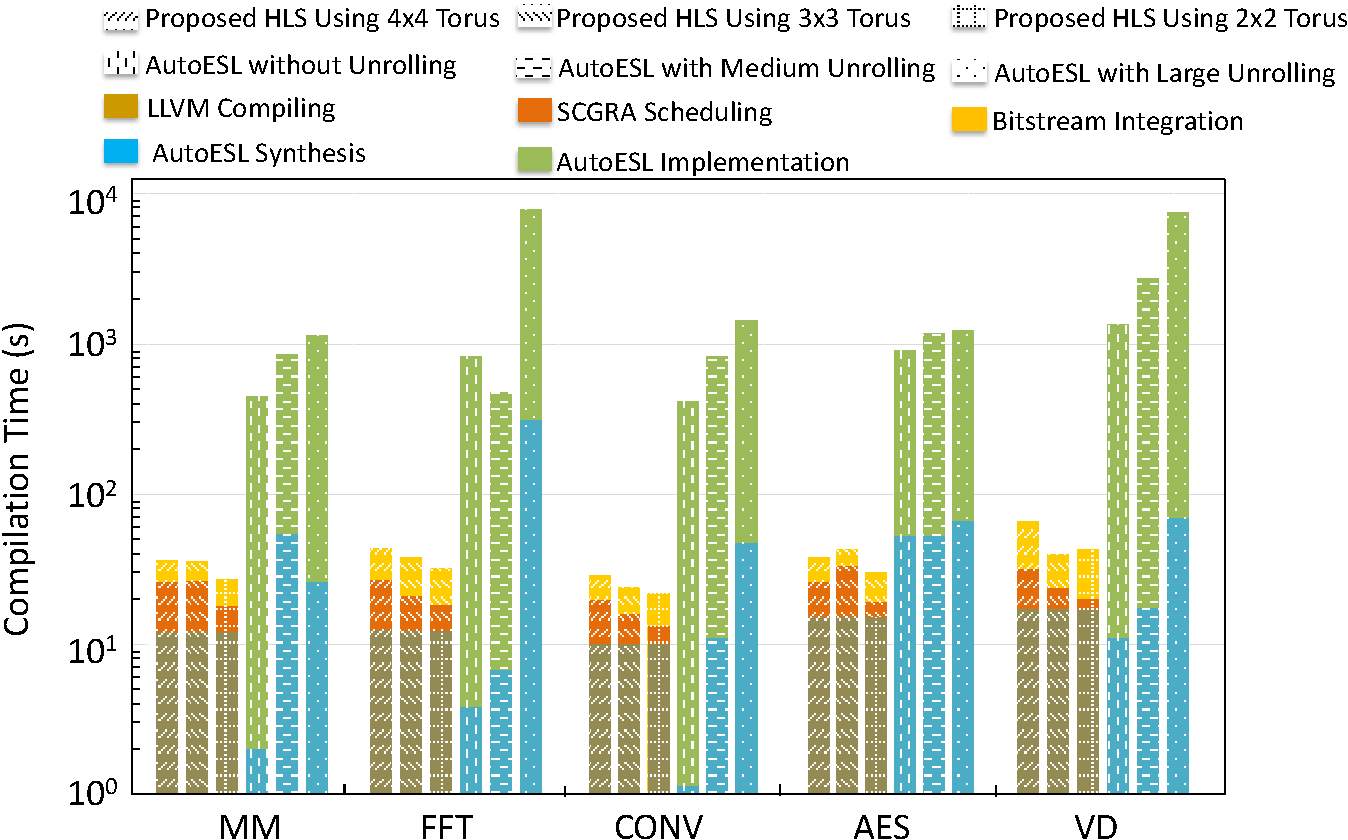
\includegraphics[width=8cm]{designtime}
\vspace{-1em}
\caption{Compilation time comparison of the benchmark using both \autoesl and the proposed HLS methodology}
\label{fig:designtime}
\vspace{-1em}
\end{figure} 

On the other hand, the proposed HLS methodology bypasses the lengthy low-level implementation steps and simply needs three high-level steps: LLVM compiling, SCGRA scheduling and bitstream integration. Each of these steps could be completed in a few seconds and implementation using this methodology is generally 10X-100X faster than even the smallest implementation using \autoesl.

\subsubsection{Hardware Implementation Efficiency}
In this section, hardware implementation including both hardware resource overhead and implementation frequency using the two design methodologies are compared.

Table \ref{tab:overhead} presents the hardware overhead of the benchmark using the proposed HLS methodology with $4 \times4$ Torus(P44), $3 \times 3$ Torus (P33), and $2 \times 2$ Torus (P22), and \autoesl with no unrolling (NUR), medium unrolling (MUR), and large unrolling (LUR). From the table, it can be seen that the proposed HLS methodology tends to use more BRAM than \autoesl does in all the occasions. The prime reason is that the proposed HLS methodology employs SCGRA as the hardware infrastructure and the SCGRA typically requires a number of large instruction memories to store all the control words (instructions). Actually, the BRAM consumption using the proposed HLS methodology roughly equals to the SCGRA scale multiplied by the scheduling result of the target application. It is also the resource bottleneck of the proposed HLS methodology. Hopefully, the context compression techniques \cite{kim2010dynamic} used in CGRA design may help remove the instruction redundancy and alleviate the BRAM requirements. While \autoesl mainly uses BRAM for buffering between different sub blocks and IO, the BRAM requirement is much lower because there are few sub blocks in the benchmark. 

\begin{table}[h]
\vspace{-1em}
\caption{Hardware overhead of the benchmark.}
\label{tab:overhead}
\centering
\small
\begin{tabular}{|c|c|c|c|c|c|c|}
\hline
\multicolumn{2}{|c|}{} & SLICE & LUT & FF & DSP & RAM\\
\hline
\multirow{4}{*}{MM} & T44 & 2273 & 4303 & 11129 & 16 & 176\\
\cline{2-7}
& T33 & 1029 & 3229 & 6958 & 9 & 99\\
\cline{2-7}
& T22 & 619 & 1045 & 2805 & 4 & 76\\
\cline{2-7}
& NUR & 158 & 296 & 320 & 1 & 2\\
\cline{2-7}
& MUR & 1151 & 3517 & 4224 & 78 & 2\\
\cline{2-7}
& LUR & 1958 & 6711 & 8006 & 182 &2\\
\hline

\multirow{4}{*}{FFT} & T44 & 2273 & 4303 & 11129 & 16 & 176\\
\cline{2-7}
& T33 & 1519 & 2574 & 6976 & 9 & 171\\
\cline{2-7}
& T22 & 619 & 1045 & 2805 & 4 & 76\\
\cline{2-7}

& NUR & 286 & 648 & 823 & 5 & 6\\
\cline{2-7}
& MUR & 595 & 1901 & 2024 & 32 & 20\\
\cline{2-7}
& LUR &	17190 &	49099 &	37283 &	654 & 20\\
\hline

\multirow{4}{*}{CONV} & T44 & 2273 & 4303 & 11129 & 16 & 176\\
\cline{2-7}
& T33 & 1029 & 3229 & 6958 & 9 & 99\\
\cline{2-7}
& T22 & 619 & 1045 & 2805 & 4 & 76\\
\cline{2-7}

& NUR &	87 & 217 & 205 & 1 & 2\\
\cline{2-7}
& MUR & 1149 & 3763 & 4558 & 98 & 2\\
\cline{2-7}
& LUR & 4213 & 13633 & 19940 & 497 & 2\\
\hline

\multirow{4}{*}{AES} & T44 & 2273 & 4303 & 11129 & 16 & 176\\
\cline{2-7}
& T33 & 1029 & 3229 & 6958 & 9 & 99\\
\cline{2-7}
& T22 & 620 & 1395 & 2817 & 4 & 108\\
\cline{2-7}

& NUR &	501 & 1251 & 1660 & 0 & 8\\
\cline{2-7}
& MUR &	705 & 1799 & 1947 & 0 &	8\\
\cline{2-7}
& LUR & 708 & 1767 & 1872 & 0 & 8\\
\hline

\multirow{4}{*}{VD} & T44 & 2782 & 4811 & 11209 & 16 & 806\\
\cline{2-7}
& T33 & 1668 & 2544 & 6325 & 9 & 387\\
\cline{2-7}
& T22 & 725 & 1298 & 2825 & 4 & 172\\
\cline{2-7}

& NUR & 1911 & 4883 & 6684 & 0 & 12\\
\cline{2-7}
& MUR & 3306 & 10033 & 12863 & 0 & 12\\
\cline{2-7}
& LUR & 8833 & 24693 & 31886 & 0 & 12\\
\hline
\end{tabular}
\vspace{-1em}
\end{table}

As for SLICE, LUT, FF and DSP, the consumption using the proposed HLS methodology mainly depends on the SCGRA scale, and it fluctuates within a narrow range when the instruction memory capacity varies. While the consumption of these components using \autoesl increases dramatically with the loop unrolling factor and it will soon eat up all the FPGA resource. When the computation kernels are not unrolled at all, \autoesl provides quite compact implementations and it consumes only a small number of SLICE, LUT, FF and DSP. When the medium loop unrolling is adopted, \autoesl and the proposed HLS methodology cost comparable number of the primitive components. When a large loop unrolling is employed, the overhead of these components using \autoesl turns to be larger than that using the proposed HLS methodology for most applications in the benchmark. The overhead comparison of AES is a bit different, because the SCGRA has more computation capability than that is required. Pre-built more light-weight SCGRA will decrease the SCGRA overhead.

Figure \ref{fig:impl_freq} shows the implementation frequency using both tools. It is clear that the SCGRAs employed in the proposed HLS methodology for all the kernels except VD are generally able to work around 400 MHz, which is close to the extreme frequency of the three-stage-pipelined DSP core implemented on the target FPGA. \autoesl has specific implementation for each benchmark, but the highest implementation frequency is only around 300MHz. When large loop unrolling is adopted, the implementation frequency deteriorates radically. The worst implementation frequency as presented in Figure \ref{fig:impl_freq} is only around 50 MHz, which offsets the performance improvement brought by the loop unrolling. Essentially, a large number of irregular blocks that randomly scatter around the FPGA using \autoesl increase the difficulty for place-and-route, causing a reduced implementation frequency. In contrast, the SCGRA is regular and well pipelined, therefore the implementation frequency is much higher. Figure \ref{fig:lib_impl_freq} displays the frequency of all the 21 SCGRA implementations. It demonstrates that the implementation frequency degrades gracefully with the increase of the SCGRA scale and instruction memory. 

\begin{figure}[h]
\centering
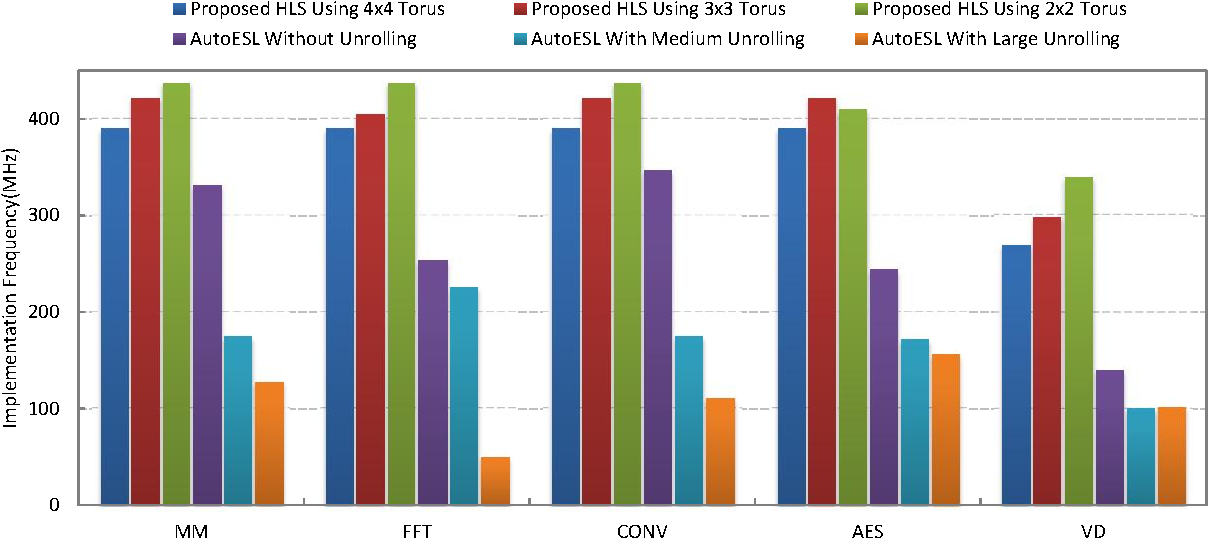
\includegraphics[width=8cm]{impl_freq}
\vspace{-1em}
\caption{Implementation frequency comparison of the benchmark using both \autoesl and the proposed HLS methodology}
\label{fig:impl_freq}
\vspace{-1em}
\end{figure}

\begin{figure}[h]
\centering
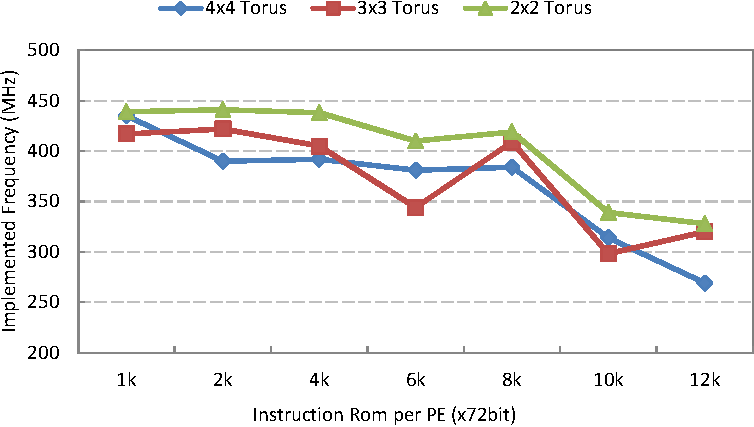
\includegraphics[width=6cm]{lib_impl_freq}
\vspace{-1em}
\caption{Implementation frequency of all the 21 SCGRAs}
\label{fig:lib_impl_freq}
\vspace{-1em}
\end{figure}


\subsubsection{Performance}
In this section, the execution time of the benchmark is taken as the metric of performance. The execution time is computed by multiplying the number of execution cycles with the implemented clock period. The number of execution cycles for \autoesl was obtained from the synthesis tools, while that of the proposed HLS methodology was obtained from the SCGRA scheduler. All clock periods of the implementations were obtained from timing reports of the final FPGA implementations.

Figure \ref{fig:sim_perf} presents the simulation performance (execution cycles) of the benchmark using both \autoesl and the proposed HLS methodology. Generally, larger loop unrolling using \autoesl leads to better simulation performance. Nevertheless, the performance gain brought by loop unrolling varies in a wide range. CONV with large loop unrolling is almost 20X faster than that without loop unrolling while AES barely benefits from the loop unrolling. The situations of MM, FFT and VD lie between the previous two extreme examples. Basically, there are three reasons for this:


First of all, single input port and single output port constrain the IO bandwidth, and potential parallel operations may be forced to be serial. This is part of the reason for all the unsatisfying performance acceleration. 

Second, \autoesl leaves the user to decide the loop unrolling. However, the design space can be extremely large and it is difficult for the user to decide the optimal unrolling factors especially under IO constrain. Take AES as an example. It consists of quite a few sub loops and \autoesl fails to unroll all the sub loops, so we have to leave some of the sub loops unchanged. These serial loops limit not only its own's execution time but also the unrolled loops in the downstream. In this case, randomly unrolling some of the sub loops may have little influence on the performance of the entire application. 

Third, source code structure may not be appropriate for \autoesl to synthesize. Take FFT as an example. FFT is a three-level nested loop, and the inner loops depend on the outmost loop. In fact, this is the reason that \autoesl fails to estimate the simulation performance. When the medium loop unrolling is adopted, we manually unroll the outmost loop into 8 stages. And it is natural to connect the 8 stage in serial manner according to the FFT structure. As each stage depends on one after another, the performance acceleration mainly relies on the overlapped computation across the stages. When the large loop unrolling scheme is employed, each stage is further unrolled. Since the neighboring stages communicate through RAM buffers which have limited IO ports, each stage still suffers the same communication bandwidth constrain and loop unrolling in a single stage is almost useless. Declaring multiple smaller vectors to guide \autoesl to synthesize more RAM buffers for communication between neighboring stages and delicately allocating the intermediate data to proper sub vectors to fully reuse the increased communication bandwidth may remove the inner communication bottleneck. Nevertheless, it is challenging for the user to reorganize the source code to fulfill such harsh requirements. In this experiment, two vectors are used to store real part and imaginary part of a complex intermediate data respectively between the neighboring stages. Therefore, it is not surprising that \autoesl fails to accelerate FFT much through the straightforward loop unrolling. 

As for the proposed HLS methodology, the performance is more predictable. According to Figure \ref{fig:sim_perf}, larger SCGRAs with more PEs generally provide higher performance and require more instruction memory while smaller SCGRAs are exactly the opposite. The only exception is VD and there are combined reasons for this. The SCGRA scheduler tends to keep load balance for better performance and operations are scattered across the SCGRA, but the parallel operations in VD are insufficient for scheduling and the communication gets more frequent. While communication in larger SCGRAs is more costly and the deep pipeline of the SCGRA makes the situation even worse, therefore, the smaller SCGRAs achieve even better performance than the larger SCGRAs. This problem can be alleviated by adjusting the scheduling strategy through slightly de-emphasizing the load balance.

\begin{figure}[h]
\centering
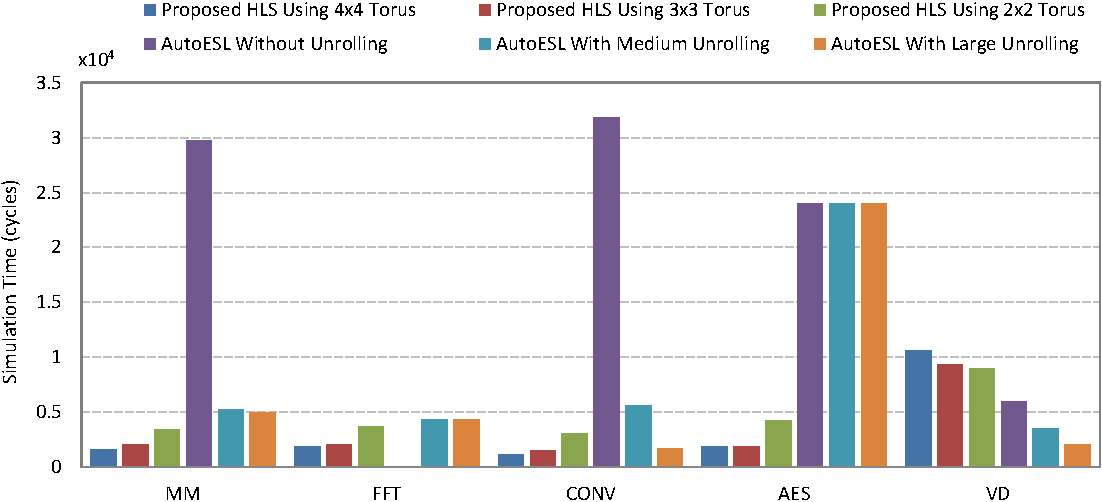
\includegraphics[width=8cm]{sim_perf}
\vspace{-1em}
\caption{Simulation performance comparison of the benchmark using both \autoesl and the proposed HLS methodology}
\label{fig:sim_perf}
\vspace{-1em}
\end{figure}

With the above analysis, we can conclude that the proposed HLS methodology outperforms \autoesl in implementing the benchmark with larger parallel computation but it is not quite effective in handling the benchmark with limited parallelism. Note that we are not denying that \autoesl is able to achieve optimal performance acceleration on FPGA. It is just difficult for the user to figure out proper source code structure and unrolling configuration for the optimal performance acceleration over such a broad design space. The proposed HLS methodology that builds SCGRA over FPGA actually scales down the design space. Meanwhile, the loops are fully unrolled and all the data dependency are completely exposed to the scheduler, so it is getting easier to find an near optimal solution. Particularly, the user simply needs to provide the SCGRA scale and maximum instruction memory depth and doesn't need to make any low level optimization decisions, which makes the design methodology more friendly to the user. 

With both the implementation frequency in Figure \ref{fig:impl_freq} and simulation performance in Figure \ref{fig:sim_perf}, the real performance of the benchmark using different HLS tools is acquired as shown in Figure \ref{fig:real_perf}. It can be seen that the proposed HLS method outperforms \autoesl in all the benchmark except VD. The highest performance of MM, FFT, CONV and AES using the proposed HLS method is around 7X, 4X, 5X and 21X faster than that using \autoesl respectively, while the performance of VD is a bit slower due to the limited parallelism and the performance acceleration is around 0.8X.

%On the other hand, the \autoesl implementations adopted RAM buffers as communication interfaces between blocks, which was incapable to provide enough bandwidth to support large parallelism exploration. Take the experiments of FFT and AES as an example. Both computation kernels of FFT and AES were divided into multiple sub-blocks to provide larger parallelism for \autoesl implementation. However, the dependent sub-blocks have to fetch data from RAM buffer in upstream and send data to RAM buffer in downstream. As a result, each sub block has additional I/O bandwidth constrains which negatively affected parallel execution. As a result, designs with larger unrolling factors failed to delivered the expected performance improvement. At the same time, the design with larger unrolling requires larger hardware resource and deteriorates the low-level implementation timing. Consequently, this has led to the performance degradation of FFT and AES with larger unrolling factors.

\begin{figure}[h]
\centering
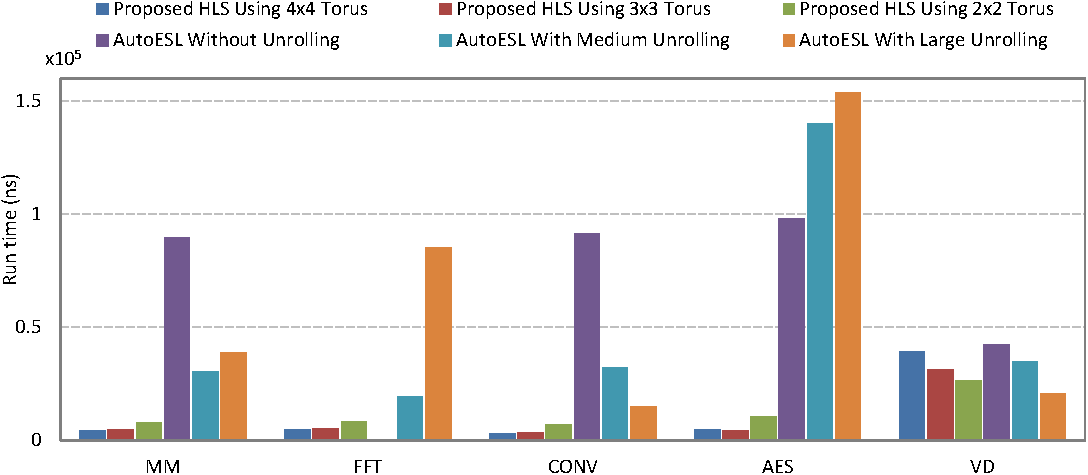
\includegraphics[width=8cm]{real_perf}
\vspace{-1em}
\caption{Performance comparison of the benchmark using both \autoesl and the proposed HLS methodology}
\label{fig:real_perf}
\vspace{-1em}
\end{figure}
